% ------------------------------------------------------------------
\renewcommand{\thisweek}{MATH327 Week 10}
\renewcommand{\moddate}{Last modified 2 May 2021}
\setcounter{section}{10}
\setcounter{subsection}{0}
\phantomsection
\addcontentsline{toc}{section}{Week 10: Interacting systems}
\section*{Week 10: Interacting systems}
\subsection{From non-interacting spins to the Ising model}
So far in this module we have considered `ideal' systems whose constituent objects do not interact with each other.
While we have seen that excellent mathematical models for real physical systems (such as stars and the cosmic microwave background) can be obtained despite this approximation of non-interacting particles, there are important statistical physics phenomena that cannot be captured by this approach.

An important class of examples, which we will investigate this week, are \textbf{phase transitions}, where interactions allow the same particles to produce extremely different large-scale behaviours, depending on control parameters such as the temperature or pressure.
An everyday example is the transition of H$_2$O molecules from liquid water to solid ice as the temperature decreases.
As the temperature of the universe itself decreased during the first few micro-seconds following the big bang, elementary particles transitioned from a so-called quark--gluon plasma to the protons and neutrons we are made out of today.
An intermediate example illustrated in the figure below (\href{https://doi.org/10.1063/PT.3.4384}{source}) involves two layers of graphene at a low temperature $T \approx 1.7$~K.
If these two layers are rotated with respect to each other by a small ``magic angle'' $\theta \approx 1.1^{\circ}$, the system transitions from being an electrical insulator to being a superconductor.

\begin{center}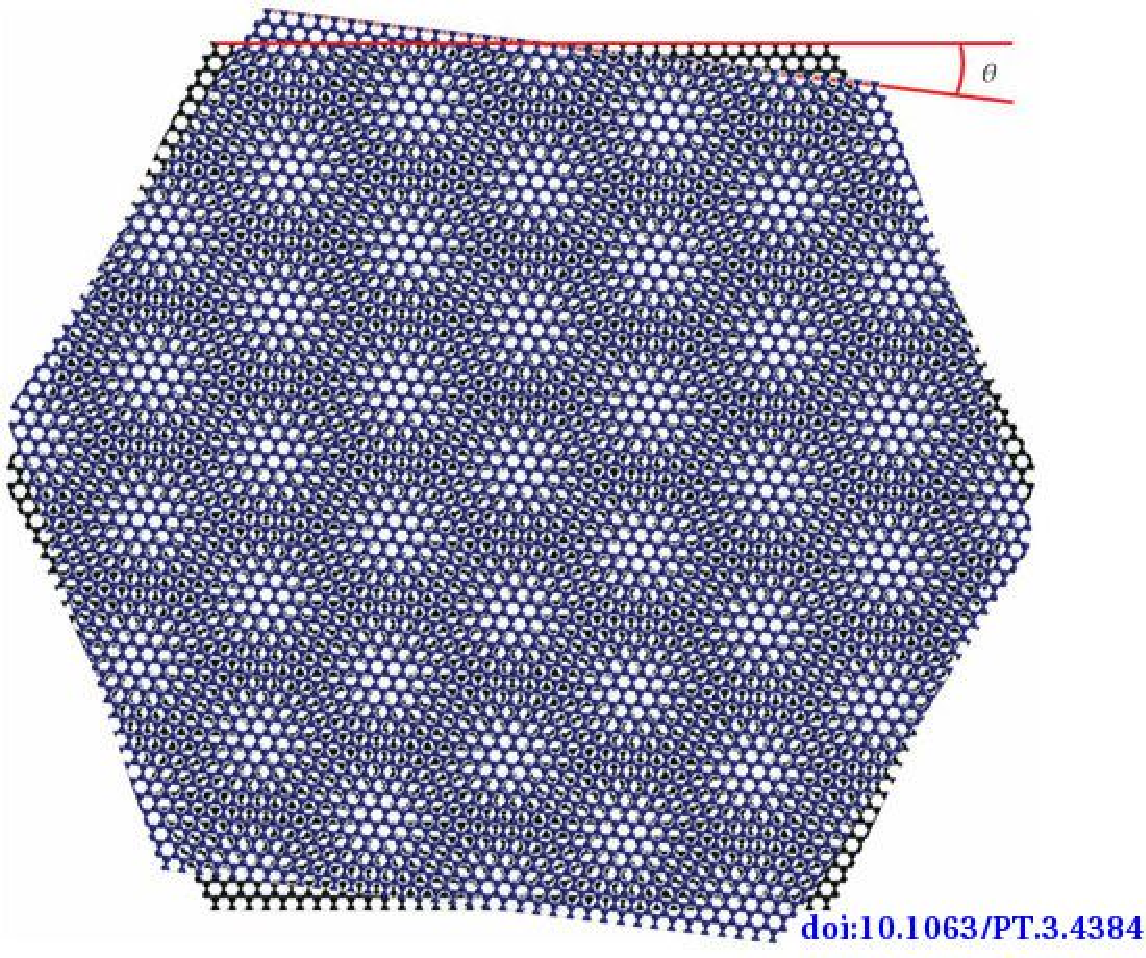
\includegraphics[width=0.5\textwidth]{figs/week10_graphene.pdf}\end{center}

We will introduce interactions and explore their effects using simple spin systems of the sort we previously analyzed in some depth during weeks $2$ and $3$.
In the non-interacting case we previously considered, the internal energy of the system (\eq{eq:spin_energy}) is
\begin{equation*}
  E = H \sum_{n = 1}^N s_n \qquad \mbox{(non-interacting)},
\end{equation*}
where $H > 0$ is the constant strength of an external magnetic field and the orientation of the $n$th spin, $s_n$, takes one of only two possible values: $s_n = 1$ if the spin is aligned anti-parallel to the field and $s_n = -1$ if the spin is aligned parallel to the field.
The ground state of the system features all $N$ spins aligned parallel to the magnetic field, with minimal energy $E_0 = -NH$.
This week we will only consider systems of distinguishable spins, which can be labeled by their fixed position in a $d$-dimensional simple cubic \textbf{lattice} like that shown below for $d = 2$ dimensions.
The $d = 1$ case of a one-dimensional lattice is precisely the system of spins arranged in a line that we analyzed in \secref{sec:spin_chain}.

\begin{center}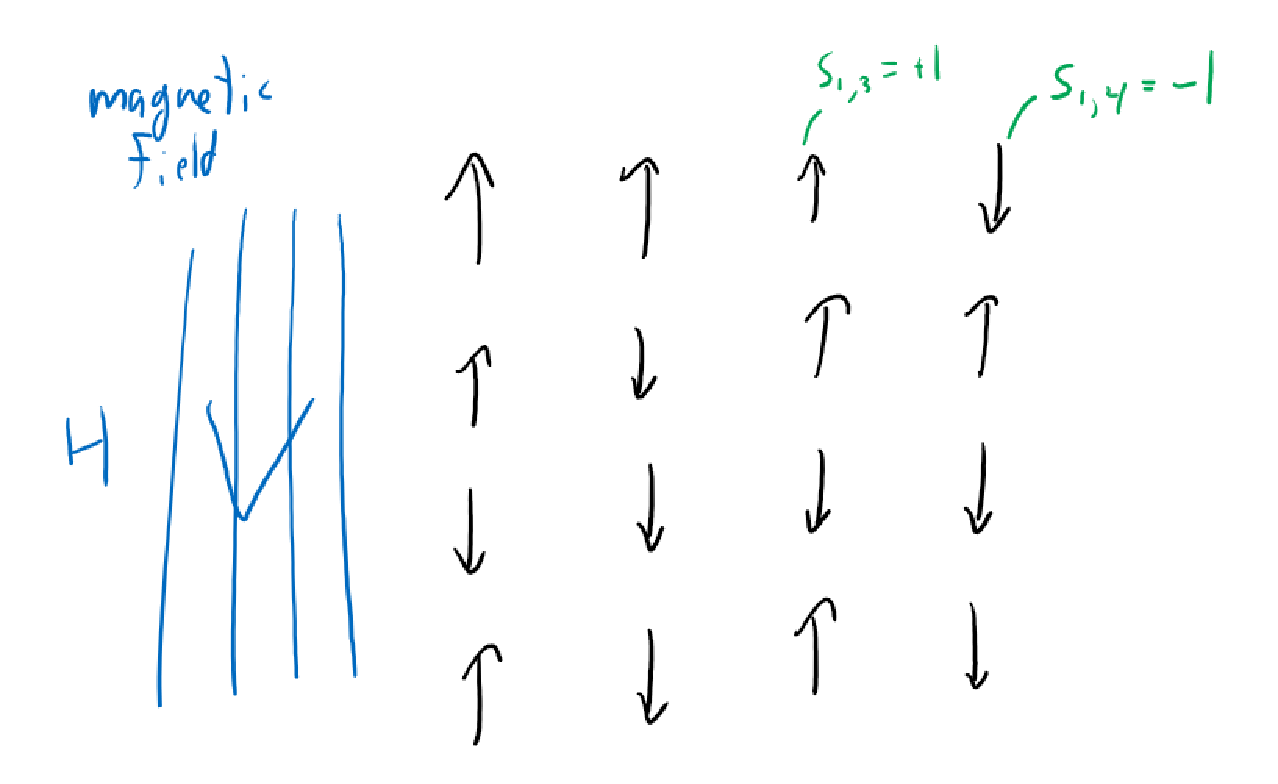
\includegraphics[width=0.8\textwidth]{figs/week10_spins.pdf}\end{center}

We can see that the total internal energy of the non-interacting system can easily be written as a sum over energies for each individual spin,
\begin{align*}
  E_n & = H s_n &
  E & = \sum_{n = 1}^N E_n \qquad \mbox{(non-interacting)}.
\end{align*}
This is a generic feature of non-interacting systems, and an aspect of the \textbf{factorization} that enormously simplifies calculations by causing the $N$-particle partition function (\eq{eq:spin_part_func}) to take the form of a product of $N$ identical terms, $Z = \left[2\cosh\left(\be H\right)\right]^N = Z_1^N$.
However, a stronger condition needs to be satisfied in order for such factorization to be guaranteed, which rigorously defines what it means for a system to be non-interacting.

\begin{shaded}
  Let $\De E_i$ be the change in the system's internal energy caused by changing its $i$th degree of freedom.
  Then the system is defined to be \textbf{non-interacting} if and only if $\De E_i$ is independent of all other degrees of freedom $k \ne i$.
\end{shaded}

For our system of $N$ distinguishable spins, the only possible change we can make to a degree of freedom is to negate it, $s_i \to -s_i$, which corresponds to flipping its alignment relative to the external magnetic field.
This spin flip causes the total energy to change,
\begin{equation*}
  E = H \sum_{n = 1}^N s_n = H\left(s_i + \sum_{k \ne i} s_k\right) \quad \lra \quad H\left(-s_i + \sum_{k \ne i} s_k\right),
\end{equation*}
corresponding to $\De E_i = -2H s_i$, which is indeed independent of all spins $s_k$ with $k \ne i$.
This simple check confirms that our definition works for the non-interacting spin system under consideration.

Now let's convert this setup into a system of interacting spins by adding the simplest possible two-spin contribution to its energy:
\begin{equation}
  \label{eq:Ising_energy}
  E = -\sum_{(ij)} s_i s_j + H \sum_{n = 1}^N s_n.
\end{equation}
The first sum runs over all pairs of nearest-neighbour spins in the lattice, denoted $(ij)$.
What is the change in energy $\De E_i$ from \eq{eq:Ising_energy} upon negating $s_i \to -s_i$?
Does this indicate an interacting or non-interacting system?
\begin{mdframed}
  \ \\[100 pt]
\end{mdframed}
The pictures below illustrate nearest-neighbour pairs for simple cubic lattices in $d = 2$ and $3$ dimensions, while also introducing some additional lattice terminology.

\begin{center}
  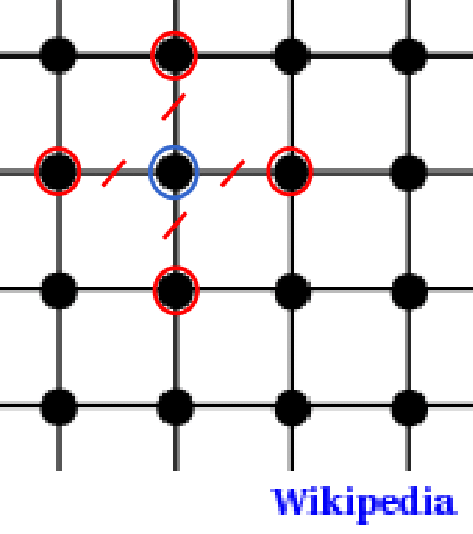
\includegraphics[height=0.4\textwidth]{figs/week10_lattice_2d.pdf}\hfill
  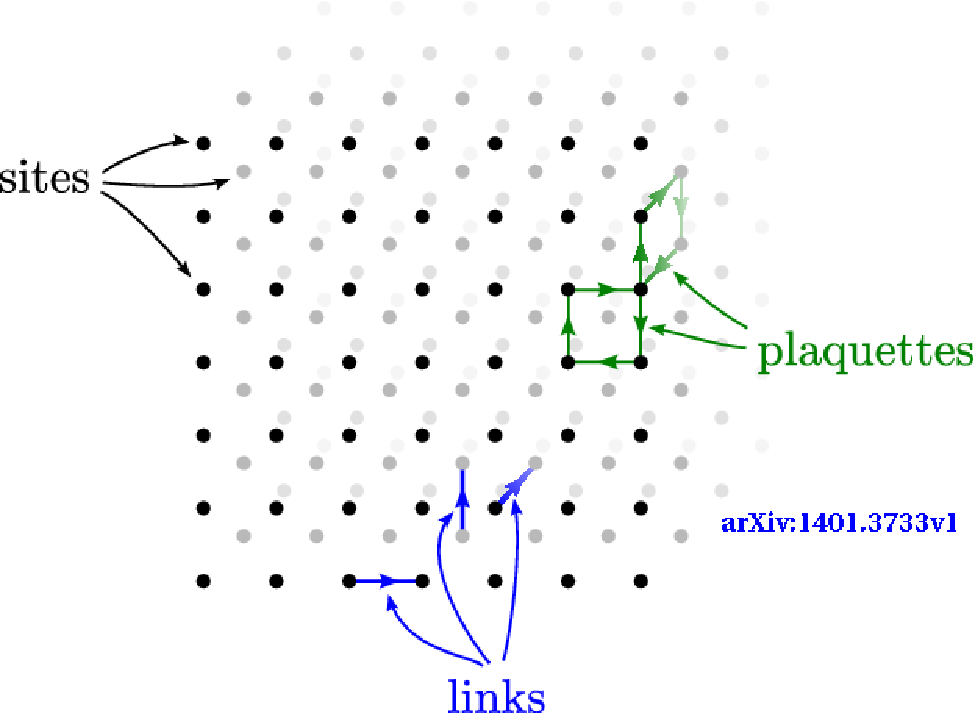
\includegraphics[height=0.4\textwidth]{figs/week10_lattice_3d.pdf}
\end{center}

Instead of drawing up- and down-pointing arrows, these pictures identify the spins with \textit{sites} in the lattice represented as points (or larger filled circles).
In simple cubic lattices, all sites are positioned in a regular grid, separated by a constant distance along each basis vector.
In between nearest-neighbour sites, we can draw \textit{links} as solid lines.
The picture of a two-dimensional lattice on the left highlights the four links (with red hatch marks) that correspond to the four nearest neighbours (circled in red) of a particular site (circled in blue).
While we can only have physical lattices with $d = 1$, $2$ or $3$ in nature, the mathematical construction works just as well for any integer $d \geq 1$.
For $d \geq 2$, an elementary unit of surface area is called a \textit{plaquettes}, while for $d \geq 3$ the elementary unit of volume is called a \textit{cube}.

Computing the energy in \eq{eq:Ising_energy} requires determining all of the nearest-neighbour pairs to be summed in the first term, which is equivalent to all of the links in the lattice, $\ell = (ij)$.
The only potential complication to this task is the need to consider what happens at the edges of the (finite) lattice.
We can avoid this complication by imposing \textbf{periodic boundary conditions}, which add an extra link between each site on the left edge of the lattice and a corresponding site on the right edge (and similarly in all other dimensions).
This is illustrated below for the simple one-dimensional lattice, which has been drawn as a circle to emphasize that all $N$ sites remain separated by a constant distance.
In higher dimensions, periodic boundary conditions produce flat (zero-curvature) $d$-dimensional tori that preserve the simple cubic lattice structure.

\begin{center}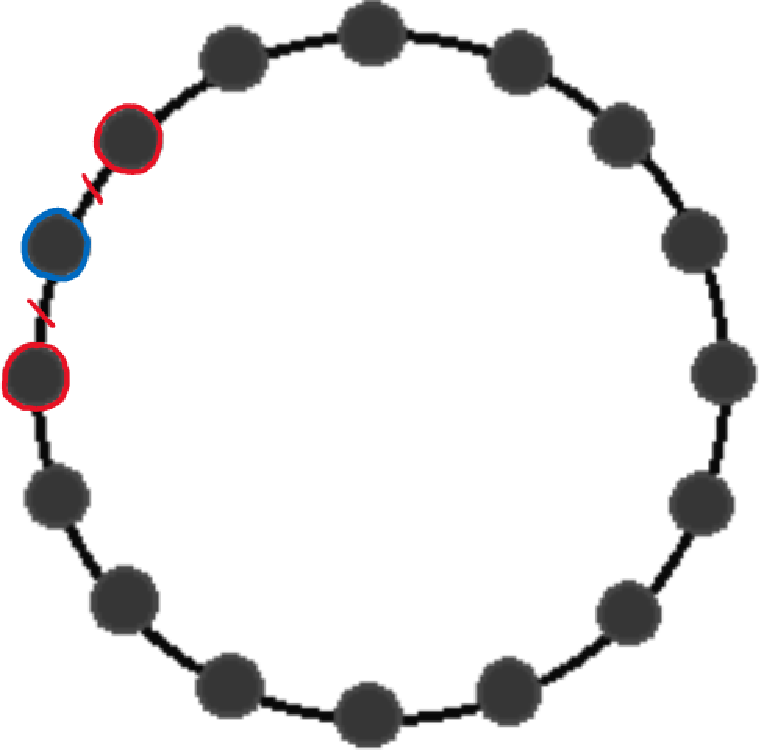
\includegraphics[width=0.45\textwidth]{figs/week10_lattice_1d.pdf}\end{center}

With periodic boundary conditions, we can easily see that the $N$-site one-dimensional lattice drawn above has $N$ links.
Each site has two links connecting it to its two nearest neighbours, and each of those links is shared between two sites, so that $\#\ell = 2N / 2 = N$.
Looking back to the two-dimensional lattice drawn farther above, the four links per site produce $\#\ell = 4N / 2 = 2N$.
How many terms are there in the sum $\sum_{(ij)}$ in \eq{eq:Ising_energy} for $N$-site lattices with periodic boundary conditions in $d$ dimensions?
\begin{mdframed}
  \ \\[50 pt]
\end{mdframed}

The energy in \eq{eq:Ising_energy}, with nearest-neighbour spins specified by the underlying simple cubic lattice structure, defines a famous system known as the $d$-dimensional \textbf{Ising model}.
Since the 1960s, the Ising model has been the basis of thousands of scientific studies analyzing everything from ferromagnetism to neural networks to urban segregation.\footnote{For a brief summary, see Charlie Wood, ``\href{https://www.quantamagazine.org/the-cartoon-picture-of-magnets-that-has-transformed-science-20200624/}{The Cartoon Picture of Magnets That Has Transformed Science}'', \textit{Quanta Magazine}, 24 July 2020.}
The model was proposed in 1920 by \href{https://en.wikipedia.org/wiki/Wilhelm_Lenz}{Wilhelm Lenz}, whose PhD student \href{https://en.wikipedia.org/wiki/Ernst_Ising}{Ernst Ising} solved the one-dimensional system as a research project in 1924.
Exactly solving the two-dimensional case (with $H = 0$) took another twenty years, culminating in renowned work by \href{https://en.wikipedia.org/wiki/Lars_Onsager}{Lars Onsager} in 1944.
The three-dimensional Ising model remains an open mathematical question, with no known exact solution.

In this context, `solving' the Ising model means deriving a closed-form expression for its canonical partition function,
\begin{equation*}
  Z(\be, N, H) = \sum_{\left\{s_n\right\}} \exp\left[-\be E(s_n)\right] = \sum_{\left\{s_n\right\}} \exp\left[\be\sum_{(ij)} s_i s_j - \be H \sum_n s_n\right].
\end{equation*}
As in \secref{sec:spin_info}, the partition function sums over all possible spin configurations $\left\{s_n\right\}$, which amounts to a sum of $2^N$ exponential factors for $N$ spins, with $\cO(N)$ terms within each exponential.
Now that the system is interacting, the partition function can no longer be factorized into $N$ identical two-term factors, making it extremely difficult to evaluate.
This is why there is no known exact solution to the three-dimensional Ising model, and it also makes `brute-force' numerical computations impractical.
Even for a system of $N = 1023$ spins (tiny compared to Avogadro's number $\sim 10^{23}$) there would be roughly $2^{1023} \sim 10^{310}$ terms in the partition function, far beyond the capabilities of existing or foreseeable supercomputers.
If we attempt `brute-force' numerical computation of every term in the partition function, even for a system of $N = 1023$ spins we would need to evaluate 
% ------------------------------------------------------------------



% ------------------------------------------------------------------
\subsection{Ising model phases and phase transition}
Similarly to how we analyzed non-interacting spin systems in \secref{sec:spin_info}, we can simplify the Ising model by considering its behaviour in the limits of high and low temperatures.
For another simplification, we will set $H = 0$ in this section, and consider
\begin{align}
  \label{eq:Ising_zero_field}
  E & = -\sum_{(ij)} s_i s_j &
  Z(\be, N) & = \sum_{\left\{s_n\right\}} \exp\left[\be\sum_{(ij)} s_i s_j\right].
\end{align}
We will see that the large-scale behaviour of the Ising model is qualitatively different at high temperatures compared to low temperatures.
In other words, the system exhibits two distinct phases for different temperatures.
This is a necessary but not sufficient condition for there to be a true phase transition---a priori, it is possible for there to be a gradual \textit{crossover} between these two phases, as opposed to a rapid transition.
We will use the Ising model to more rigorously define what exactly constitutes a phase transition, and how this can be distinguished from a crossover.

The Ising model partition function becomes extremely simple in the \textbf{high-temperature} limit $\be \to 0$.
What is its asymptotic limit?
\begin{mdframed}
  $\displaystyle Z(\be = 0, N) = $ \\[50 pt]
\end{mdframed}
You should find a result identical to that for a micro-canonical system with energy $E = 0$, which is clearly non-interacting since $\De E_i = 0$.
Every spin configuration is a different micro-state of the system, all with the same probability $p_i = 1 / 2^N$, as in \eq{eq:micro_equil}.

Effectively, we are considering temperatures so high that the energy from \eq{eq:Ising_zero_field} is negligible for any spin configuration.
Although the energy no longer distinguishes between different micro-states, we can define a quantity that continues to be sensitive to the details of the spin configuration.
This is the \textbf{magnetization} $M = n_+ - n_-$, where we redefine $n_{\pm}$ to be the number of spins with value $\pm 1$, so that $N = n_+ + n_-$.\footnote{In week $2$ we defined $n_{\pm}$ based on spins' alignment with or against the external magnetic field, which no longer applies now that we have set $H = 0$.}
It is convenient to normalize the total magnetization $M$ by the number of spins,
\begin{equation}
  \label{eq:Ising_magnet}
  |m| \equiv \frac{|M|}{N} = \frac{|n_+ - n_-|}{n_+ + n_-}
\end{equation}
so that $0 \leq |m| \leq 1$ for any value of $N$.

Our task is now to determine the expectation value of the magnetization at high temperatures.
Above we found that all spin configurations are equally probable in this regime, so $\vev{|m|}$ will be determined by how likely it is for these micro-states to have a particular magnetization.
For example, there are only two micro-states with $|m| = 1$, corresponding to $(n_+, n_-) = (N, 0)$ and $(0, N)$.
In general, just as we saw in \eq{eq:spin_states}, there are
\begin{equation*}
  \binom{N}{n_+} = \binom{N}{n_-} = \frac{N!}{n_+! \; n_-!}
\end{equation*}
equally probable micro-states with a given $n_+ = N - n_-$.
For large $N \gg 1$ this binomial coefficient is factorially peaked around
\begin{equation*}
  n_+ = n_- = \frac{1}{2} N \qquad \lra \qquad |m| = 0,
\end{equation*}
which defines a \textbf{disordered phase} with similar numbers of up- and down-pointing spins producing a small magnetization.
In the so-called \textit{thermodynamic limit} $N \to \infty$, the expectation value of the magnetization in the disordered phase vanishes exactly, $\vev{|m|} \to 0$.

We now need to determine $\vev{|m|}$ in the \textbf{low-temperature} limit $\be \to \infty$.
In this regime, as we saw in \secref{sec:spin_chain}, the Boltzmann factor $\exp\left[\be\sum_{(ij)} s_i s_j\right]$ makes it exponentially more likely for the system to adopt micro-states with lower energies.
In particular, we can expect the ground state to dominate the expectation value of the magnetization, $\vev{|m|}$, up to exponentially suppressed corrections from higher-energy excited states.
With $H = 0$, the Ising model has two degenerate ground states corresponding to the two ways all the spins can be aligned with each other: $(n_+, n_-) = (N, 0)$ and $(0, N)$.
What is the ground-state energy of the $N$-site Ising model in $d$ dimensions?
\begin{mdframed}
  $\displaystyle E_0 = -\sum_{(ij)} s_i s_j = $ \\[50 pt]
\end{mdframed}

As mentioned above, both of these degenerate ground states have the maximal magnetization $|m| = 1$.
Let's check what effect the first excited state would have on the overall magnetization of the system.
The first excited state involves negating (or `flipping') a single spin, corresponding to $(n_+, n_-) = (N - 1, 1)$ and $(1, N - 1)$.
Because any one of the $N$ spins in the lattice could be flipped, the degeneracy of the first excited state grows with $N$:
\begin{equation*}
  \binom{N}{1} + \binom{N}{N - 1} = 2N.
\end{equation*}
At the same time, as $N$ increases the magnetization of each of these micro-states gets closer to that of the ground state,
\begin{equation*}
  |m| = \frac{N - 1}{N} = 1 - \frac{1}{N}.
\end{equation*}
The key factor is the probability for the system to be in one of these micro-states, which depends on the energy of the first excited state, $E_1$.
What is the first-excited-state energy of the $N$-site Ising model in $d$ dimensions?
\begin{mdframed}
  $\displaystyle E_1 = $ \\[100 pt]
\end{mdframed}

Let's put things together by computing the relative probability for the $d$-dimensional Ising model to be in its ground state with $|m| = 1$ compared to its first excited state with $|m| = 1 - \frac{1}{N}$, accounting for the different number of micro-states in each case:
\begin{equation*}
  \frac{p(E_0)}{p(E_1)} = \frac{2\cdot \exp\left[\be d\cdot N\right]}{2N\cdot \exp\left[\be \left(d\cdot N - 4d\right)\right]} = \frac{\exp\left[4\be d\right]}{N}.
\end{equation*}
For any fixed $N$, a sufficiently low temperature will cause the ground state to dominate.
This defines an \textbf{ordered phase} in which essentially all spins are aligned in the same direction, producing a large expectation value for the magnetization, $\vev{|m|} = 1$.

We have seen that the magnetization $\vev{|m|}$ distinguishes between the high- and low-temperature behaviour of the $d$-dimensional Ising model.
In the high-temperature disordered phase, the magnetization is small and $\vev{|m|} \to 0$ in the thermodynamic limit $N \to \infty$.
In the low-temperature ordered phase, the magnetization is large and $\vev{|m|} \to 1$ as $T \to 0$.
This is typical behaviour for interacting statistical systems, where the quantity distinguishing between these two phases (here the magnetization) is known as the \textbf{order parameter}.
The behaviour of the order parameter is what distinguishes gradual crossovers from rapid phase transitions.

\begin{shaded}
  A phase transition is characterized by a discontinuity in the order parameter or its derivative(s), in the $N \to \infty$ thermodynamic limit.
  The value(s) of the control parameter(s) at which the discontinuity occurs define the \textit{critical point} corresponding to the transition.
\end{shaded}

For the zero-field ($H = 0$) Ising model, the control parameter is the temperature $T$, and any phase transition would occur at a \textbf{critical temperature} $T_C$.
The sketches below illustrate the most common types of phase transitions.
When the order parameter (OP) itself is discontinuous (shown by a dashed line), the transition is said to be a \textit{first-order} phase transition.
When the order parameter is continuous at $T_C$ but its first derivative is discontinuous, the transition is said to be a \textit{second-order} phase transition.
This naming scheme generalizes to higher-order phase transitions, the most remarkable of which is the infinite-order BKT phase transition (named after \href{https://en.wikipedia.org/wiki/Vadim_Berezinskii}{Vadim Berezinskii}, \href{https://en.wikipedia.org/wiki/J._Michael_Kosterlitz}{J.\ Michael Kosterlitz} and \href{https://en.wikipedia.org/wiki/David_J._Thouless}{David Thouless}), which was awarded the 2016 Nobel Prize in Physics.

\begin{center}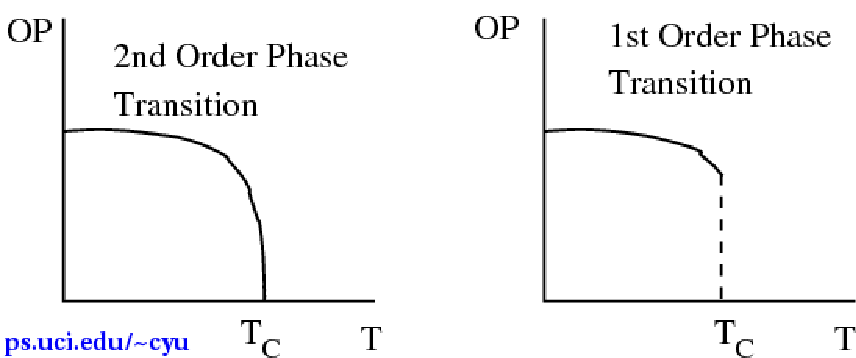
\includegraphics[width=0.8\textwidth]{figs/week10_transitions.pdf}\end{center}

Because true discontinuities are only possible with an infinite number of degrees of freedom, it is really the way in which the system approaches the $N \to \infty$ thermodynamic limit that distinguishes crossovers from true phase transitions.
We will conclude this week's consideration of interacting systems by developing a useful approximation for the Ising model, which will turn out to be more reliable as the dimensionality $d$ increases.
% ------------------------------------------------------------------



% ------------------------------------------------------------------
\subsection{The mean-field approximation}
Looking back to \eq{eq:Ising_magnet}, we can identify the magnetization (with no absolute value) as the average spin,
\begin{equation*}
  m = \frac{M}{N} = \frac{1}{N}\left(n_+ - n_-\right) = \frac{1}{N} \sum_{n = 1}^N s_n.
\end{equation*}
The `mean' in the mean-field approximation refers to the expectation value of the average spin,
\begin{equation*}
  \vev{m} = \frac{1}{Z} \sum_{\left\{s_n\right\}} m \; e^{-\be E(s_n)} = \frac{1}{N} \sum_{n = 1}^N \vev{s_n},
\end{equation*}
which is independent of the spin configuration $\left\{s_n\right\}$ and is simply a function of the inverse temperature \be and magnetic field strength $H$.\footnote{To be consistent with the redefinition of $n_{\pm}$ above \eq{eq:Ising_magnet}, we reverse our sign convention for the magnetic field, $H \to -H$.}
By adding and subtracting factors of $\vev{m}$, we can exactly rewrite each nearest-neighbour term in the Ising model energy, \eq{eq:Ising_energy}, as
\begin{align}
  s_i s_j & = \left[\left(s_i - \vev{m}\right) + \vev{m}\right] \times \left[\left(s_j - \vev{m}\right) + \vev{m}\right] \cr
          & = \left(s_i - \vev{m}\right) \left(s_j - \vev{m}\right) + \left(s_i + s_j\right)\vev{m} - \vev{m}^2. \label{eq:MF_start}
\end{align}

The factors of $\left(s_i - \vev{m}\right)$ correspond to the spins' fluctuations around their mean value $\vev{m}$.
By conjecturing that these fluctuations are small \textit{on average}, we can approximate the Ising model energy by neglecting the first term in \eq{eq:MF_start} when summing over all links:
\begin{equation*}
  E = -\sum_{(ij)} s_i s_j - H \sum_{n = 1}^N s_n \quad \lra \quad \EMF = -\sum_{(ij)} \left[\left(s_i + s_j\right)\vev{m} - \vev{m}^2\right] - H \sum_{n = 1}^N s_n.
\end{equation*}
The sum over the links $\ell = (ij)$ in $d$ dimensions simply counts $d\cdot N$ factors of the constant $\vev{m}^2$.
Similarly, since the first term includes both spins $\left(s_i + s_j\right)$ on each end of the link, every individual spin appears $2d$ times in the sum over links, which we can combine with the sum over sites:
\begin{equation}
  \label{eq:MF_energy}
  \EMF = d\cdot N \vev{m}^2 - \left(2d\vev{m} + H\right) \sum_{n = 1}^N s_n \equiv d\cdot N \vev{m}^2 - H_{\text{eff}} \sum_{n = 1}^N s_n,
\end{equation}
\newpage % WARNING: FORMATTING BY HAND
\noindent defining an effective magnetic field $H_{\text{eff}}$ that depends on the mean spin.
What is the change in energy $\De E_i$ from \eq{eq:MF_energy} upon negating $s_i \to -s_i$?
Does this indicate an interacting or non-interacting system?
\begin{mdframed}
  \ \\[100 pt]
\end{mdframed}

The mean-field approximation producing \eq{eq:MF_energy} makes it very easy to compute the corresponding canonical partition function
\begin{align}
  \ZMF & = \sum_{\left\{s_n\right\}} \exp\left[-\be E(s_n)\right] = \exp\left[-\be d\cdot N \vev{m}^2\right] \sum_{s_1 = \pm 1} \cdots \sum_{s_N = \pm 1} \exp\left[-x \sum_{n = 1}^N s_n\right] \cr
       & = \exp\left[-\be d\cdot N \vev{m}^2\right] \left(2\cosh\left[\be H_{\text{eff}}\right]\right)^N \nonumber \\
       & = \exp\left[-\be d\cdot N \vev{m}^2\right] \left(2\cosh\left[\be \left(2d\vev{m} + H\right)\right]\right)^N,
\end{align}
where we defined $x = -\be H_{\text{eff}}$ to put the sums into exactly the same form as \eq{eq:spin_part_func}.
We see that the mean-field partition function exhibits complicated dependence on $\vev{m}$.
In order to get a handle on this dependence, we need to determine another relation between $\vev{m}$ and $\ZMF$.

We can do this by recalling the connection between the magnetization and the average spin discussed at the start of this section.
Because the total $N$-spin magnetization
\begin{equation*}
  M = n_+ - n_- = \sum_{n = 1}^N s_n,
\end{equation*}
we can write the full Ising model energy as
\begin{equation*}
  E = -\sum_{(ij)} s_i s_j - H \sum_{n = 1}^N s_n = -\sum_{(ij)} s_i s_j - H M,
\end{equation*}
with corresponding canonical partition function
\begin{equation*}
  Z = \sum_{\left\{s_i\right\}} \exp\left[\be \sum_{(ij)} s_i s_j + \be H M\right].
\end{equation*}
\newpage % WARNING: FORMATTING BY HAND
\noindent From our earlier experience with the canonical ensemble, it now comes as no surprise that $\vev{M} = N\vev{m}$ can be related to a derivative of the Helmholtz free energy $F = -T\log Z$.
What is this relation?
\begin{mdframed}
  $\displaystyle \pderiv{}{H} F = $ \\[100 pt]
\end{mdframed}

Returning to the mean-field approximation,
\begin{equation*}
  \log \ZMF = N\log \cosh\left[\be \left(2d\vev{m} + H\right)\right] + \left\{H\mbox{-independent terms}\right\},
\end{equation*}
we can use this relation between $\vev{m}$ and $\ZMF$ to find
\begin{equation*}
  \vev{m} = \frac{1}{N\be} \pderiv{}{H}\log \ZMF = \frac{1}{\be} \frac{1}{\cosh\left[\be \left(2d\vev{m} + H\right)\right]} \pderiv{}{H}\cosh\left[\be \left(2d\vev{m} + H\right)\right].
\end{equation*}
Simplifying, we obtain a \textbf{self-consistency condition} for the magnetization in the mean-field approximation:
\begin{equation}
  \label{eq:consistency}
  \vev{m} = \tanh\left[\be \left(2d\vev{m} + H\right)\right].
\end{equation}
Solving this equation for $\vev{m}$ is equivalent to finding the roots of the equation $\tanh\left[\be (2d\cdot x + H)\right] - x = 0$.

A straightforward way to inspect such solutions is by plotting both
\begin{align*}
  f(\vev{m}) & = \vev{m} &
  g(\vev{m}) & = \tanh\left[\be (2d\vev{m} + H)\right]
\end{align*}
and monitoring the intersections of these two functions.
Fixing $d = 2$ dimensions, the plot below considers the simplest case $\be = \frac{1}{4}$ and $H = 0$ for which $g(\vev{m}) = \tanh\left[\vev{m}\right]$ (the solid line).
There is only a single intersection between this function and $f(\vev{m})$ (the dashed line), at $\vev{m} = 0$.

\begin{center}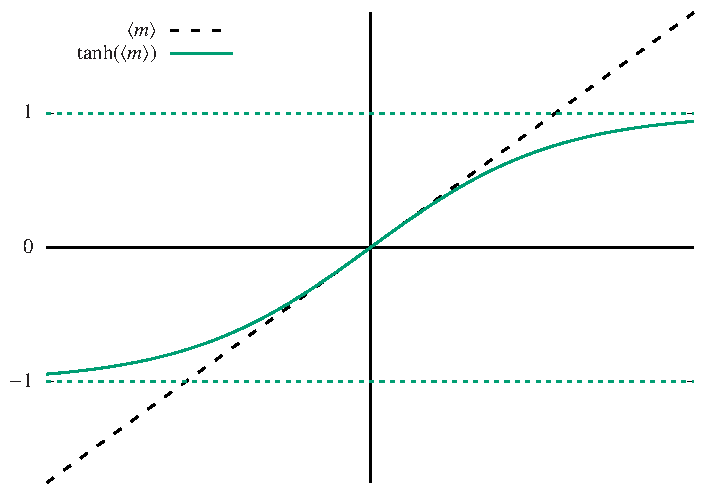
\includegraphics[width=0.7\textwidth]{figs/week10_consistency.pdf}\end{center}

Before interpreting this result, let's check how the intersections depend on \be and $H$.
In the next plot below we keep the same temperature $T = 1 / \be = 4$ while turning the external magnetic field back on.
A positive $H > 0$ simply shifts $g(\vev{m})$ to the left (the green line), while a negative $H < 0$ shifts it to the right (the blue line).
For $H = \pm 2$, there is still only a single intersection, at $\vev{m} \approx \pm 0.88$.
We can see that because $-1 \leq \tanh x \leq 1$, the mean-field self-consistency condition can only ever predict $-1 \leq \vev{m} \leq 1$, in accord with the definition of the magnetization.

\begin{center}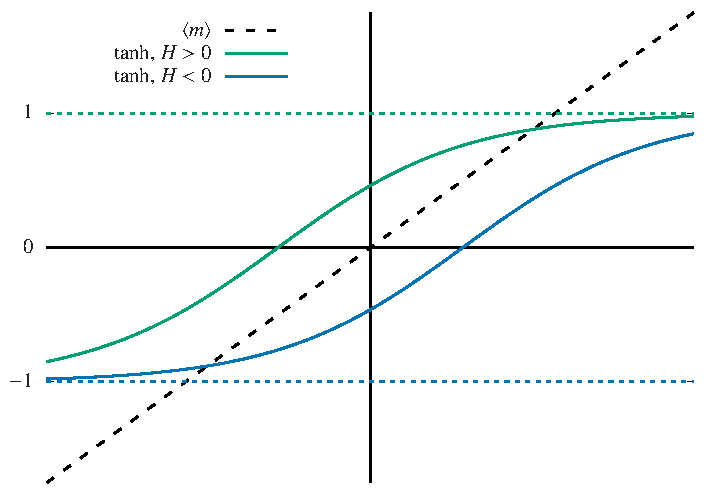
\includegraphics[width=0.7\textwidth]{figs/week10_consistency_H.pdf}\end{center}

Next, if we decrease the temperature, $g(\vev{m})$ becomes steeper, more rapidly interpolating between those limiting values $-1 \leq \tanh x \leq 1$.
The plot below illustrates this for $T = 1 / \be = 2$, so that $\be = \frac{1}{2}$ is doubled.
Already for this temperature and magnetic field $H = \pm 2$, the intersection is $\vev{m} \approx \pm 1$ to a very good approximation.
We can interpret this result as an indication that the system is in an ordered phase where all spins are aligned with the external field.

\begin{center}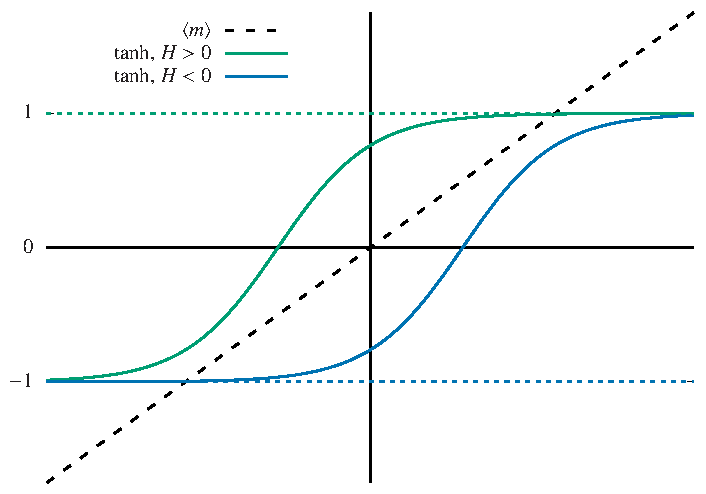
\includegraphics[width=0.7\textwidth]{figs/week10_consistency_H-beta.pdf}\end{center}

To search for a phase transition we need to turn off that external field by setting $H = 0$, and consider how the solutions of the self-consistency condition depend on the temperature.
We do this in the next plot below, considering a low temperature $T = 2$ with $\be = \frac{1}{2}$ (the red line), the same green curve for $T = 4$ shown in the first plot above, and a high temperature $T = *$ with $\be = \frac{1}{8}$ (the blue line).
While the $\vev{m} = 0$ expected in the disordered phase is always a possible solution, something interesting happens at lower temperatures, where the steeper $\tanh$ function introduces two additional solutions at $\vev{m} = \pm m_0$.
As $T \to 0$, this $m_0 \to 1$, approaching the magnetization of the ordered phase.

\begin{center}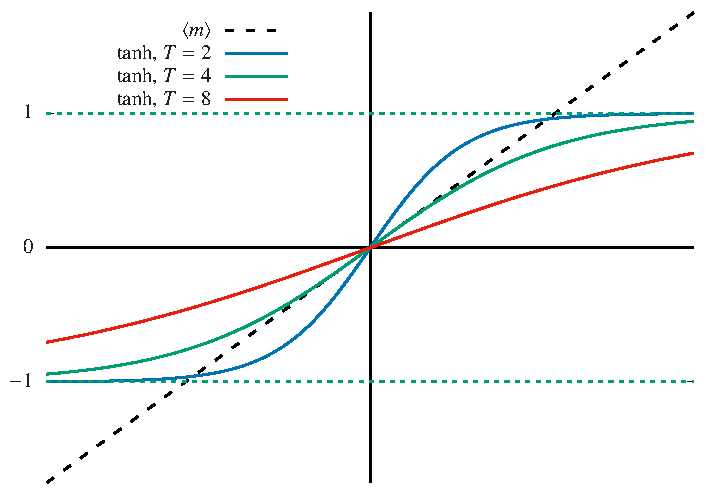
\includegraphics[width=0.7\textwidth]{figs/week10_consistency_beta.pdf}\end{center}

When there are three solutions $\vev{m} = \left\{-m_0, 0, m_0\right\}$ at low temperatures, we can determine that the $\vev{m} = 0$ solution is actually \textit{unstable}.
In this case, the slope of the $\tanh$ at $\vev{m} = 0$ must be greater than $1$.
Any positive value $\vev{m} = \varepsilon > 0$ would therefore produce $\tanh\left[2\be d\vev{m}\right] > \vev{m}$, violating the self-consistency condition in \eq{eq:consistency}.
Since the violation comes from $\vev{m}$ being too small compared to the $\tanh$, $\vev{m}$ would be driven to increase further, until it eventually reached the non-zero solution $\vev{m} = m_0$.
The analogous argument implies any negative value $\vev{m} = -\varepsilon < 0$ would drive $\vev{m}$ away from zero and to the $\vev{m} = -m_0$ solution.

This argument can be visualized by plotting $\tanh\left[2\be d\vev{m}\right] - \vev{m}$ vs.\ $\vev{m}$ as shown in the final plot below.
Whenever this difference is negative, it implies $\vev{m}$ is larger than the self-consistency condition allows, and therefore consistency requires reducing $\vev{m}$, shown by arrows pointing to the left.
Conversely, whenever the difference is positive, $\vev{m}$ would have to increase to recover consistency, shown by the arrows pointing to the right.
For the low temperature $T = 2$, we see that the arrows move the system away from the unstable solution $\vev{m} = 0$ and to the stable solutions $\vev{m} = \pm m_0$.

\begin{center}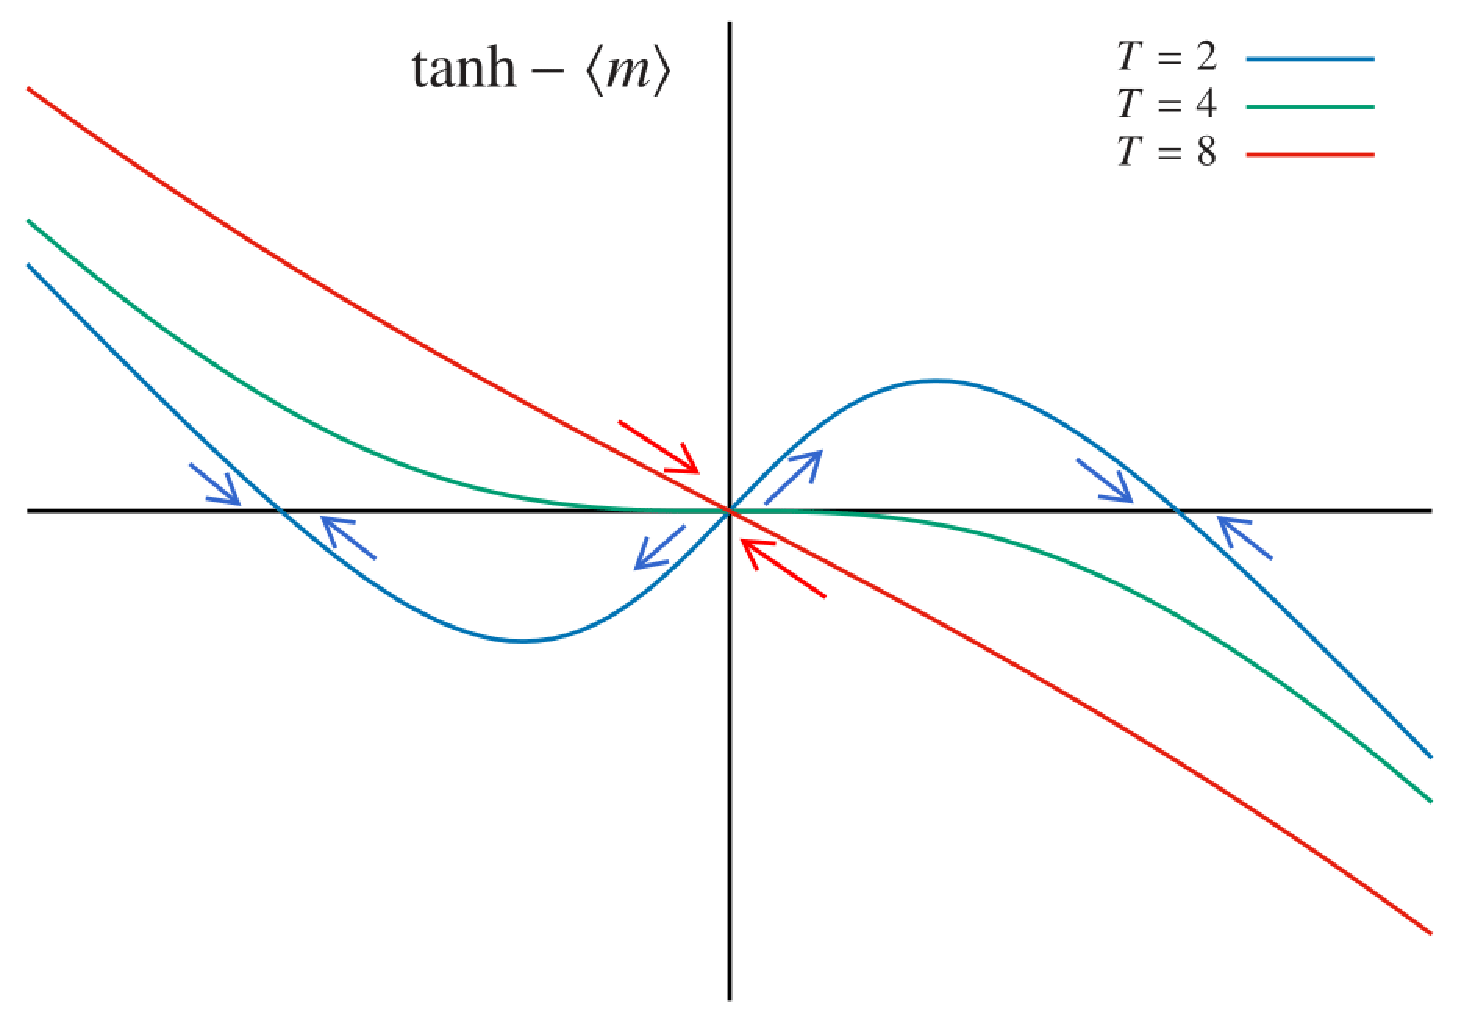
\includegraphics[width=0.7\textwidth]{figs/week10_consistency_flow.pdf}\end{center}

Reassuringly, the mean-field approximation with $H = 0$ therefore reproduces the behaviour we derived in the previous section.
For high temperatures we have $\vev{m} = 0$ consistent with the disordered phase, while for low temperatures we have $|\vev{m}| = m_0 \to 1$ consistent with the ordered phase.
We can also determine the temperature at which the $\vev{m} = \pm m_0$ solutions appear and the $\vev{m} = 0$ solution becomes unstable.
As described above, this occurs whenever the slope of the $\tanh$ function at $\vev{m} = 0$ is greater than $1$.
Using $\tanh(x) = x + \cO\left(x^3\right)$ for $x \approx 0$, what is the slope of this $\tanh$?
\begin{mdframed}
  $\displaystyle \left. \frac{d}{d\vev{m}} \tanh\left[2\be d\vev{m}\right]\right|_{\vev{m} = 0} = $ \\[50 pt]
\end{mdframed}

You should find that the change from the high-temperature disordered phase to the low-temperature ordered phase occurs at $T_c = 2d$ in $d$ dimensions, or equivalently $\be_c = \frac{1}{2d}$.
Despite the subscript, we don't yet know if this $T_c$ is a true critical temperature.
In order to check whether the mean-field approximation of the $H = 0$ Ising model predicts a crossover or a true phase transition, we need to check whether or not the order parameter $\vev{m}$ or its derivatives are discontinuous at $T_c$.
We can do this by considering the self-consistency condition for a temperature $T = 1 / \be$ lower than but close to $T_c = 2d$, which would produce $0 < |\vev{m}| \ll 1$ and allow us to expand
\begin{equation*}
  \vev{m} = \tanh\left[\frac{2d}{T} \vev{m}\right] \approx \frac{T_c}{T} \vev{m} - \frac{1}{3}\left(\frac{T_c}{T} \vev{m}\right)^3.
\end{equation*}
What is the resulting prediction for $\vev{m}$?
\begin{mdframed}
  \ \\[100 pt]
\end{mdframed}

Approximating $\frac{T}{T_c} \approx 1$, your result should resemble
\begin{equation*}
  \vev{m} = \pm \sqrt{3} \left(\frac{T_c - T}{T_c}\right)^{1 / 2} \qquad \mbox{for } \ T \lesssim T_c.
\end{equation*}
From this, we can see that the order parameter $\vev{m}$ is continuous at $T_c$:
\begin{equation}
  \vev{m} \propto \left\{\begin{array}{cl} \left(T_c - T\right)^{1 / 2} & \mbox{for } \ T \lesssim T_c \\[3 pt]
                                           0                            & \mbox{for } \ T \gtrsim T_c\end{array}\right. .
\end{equation}
However, its first derivative
\begin{equation*}
  \frac{d\vev{m}}{dT} \propto \frac{1}{\left(T_c - T\right)^{1 / 2}}
\end{equation*}
diverges as $T \to T_c$ from below, predicting a second-order phase transition with critical temperature $T_c = 2d$ in $d$ dimensions.
The power-law dependence $\vev{m} \propto \left(T_c - T\right)^b$ is a generic feature of second-order phase transitions, where the power $b$ is known as a \textbf{critical exponent}, in this case $b = 1 / 2$.

At this point we have invested some effort to find that the mean-field approximation of the $d$-dimensional Ising model, with $H = 0$, predicts a second-order phase transition at $T_c = 2d$ with critical exponent $1 / 2$.
Let's wrap up by quickly checking the reliability of the mean-field approximation and the accuracy of these results it has given us.

The accuracy of the mean-field results turns out to depend on the number of dimensions.
For the one-dimensional ($d = 1$) Ising model that Ising himself solved, there is no phase transition at all.\footnote{You can find the exact solution of the one-dimensional Ising model in Section~5.3.1 of David Tong's \href{https://www.damtp.cam.ac.uk/user/tong/statphys.html}{\textit{Lectures on Statistical Physics}} (reference~1 in the list of further reading on page~6).}
The mean-field approximation fails badly in this case.

The situation improves for the two-dimensional Ising model.
Onsager's exact $H = 0$ solution reveals a second-order phase transition, with inverse critical temperature $\be_c = \frac{1}{2} \log\left(1 + \sqrt{2}\right) \approx 0.44$ and $\vev{m} \propto \left(T_c - T\right)^{1 / 8}$ for $T \lesssim T_c$ corresponding to a critical exponent $1 / 8$.
While the mean-field approach now provides the correct qualitative behaviour, its prediction $\be_c = \frac{1}{2d} = 0.25$ is off by almost a factor of $2$, while the mean-field critical exponent $b = 1 / 2$ is four times larger than the true $b = 1 / 8$.

For higher dimensions $d \geq 3$ there is no known exact solution for the Ising model, but the existence of a second-order phase transition can be established, while the corresponding critical temperature and critical exponents can be computed numerically.
In three dimensions the mean-field $T_c = 2d = 6$ and $b = 1 / 2$ are still only rough first approximations to the true $T_c \approx 4.5$ and $b \approx 0.32$. % From arXiv:1304.4110 and Tong
The mean-field prediction for the critical exponent $b = 1 / 2$ turns out to be correct for $d \geq 4$, while the critical temperature $T_c = 2d$ gradually approaches the true value as the number of dimensions increases.
(Numerical computations find $T_c \approx 6.7$, $8.8$, $10.8$ and $12.9$ for $d = 4$, $5$, $6$ and $7$, respectively.) % From arXiv:1202.3031 and arXiv:1502.07613
Formally, the mean-field approximation exactly reproduces the Ising model in the unphysical limit of infinite dimensions, $d \to \infty$.
Roughly speaking, the greater reliability of the mean-field approach in higher dimensions is due to the larger number of nearest neighbours for each site, $2d$, which allow that site to interact with a better approximation to the mean spin.
% ------------------------------------------------------------------
